\font\jhhei="Microsoft JhengHei"
\font\Title="Heiti TC" at 18pt
\font\Section="Heiti TC" at 14pt
\font\Subsection="Heiti TC" at 12pt
\font\xesl="FreeSerif/I"
\font\ComputerModernTypewritter="[/usr/share/fonts/X11/Type1/Type1/sftt1000.pfb]"

\newcommand{\xett}{\ComputerModernTypewritter}
\newcommand\titlename{数字图像处理第一次作业}
\newcommand\vicetitle{}
\newcommand{\myauthor}{@Fanchy\_Lee}

\documentclass[a4paper,10pt]{article}
\usepackage[top=1in, bottom=1.2in, left=1.25in, right=1.25in]{geometry}
\usepackage{url}
\usepackage{titlesec} 
\usepackage{natbib} 
\usepackage{amsthm,amsmath,yhmath} 
\usepackage{graphicx,caption2} 
\usepackage{amssymb} 
\usepackage{indentfirst} 
\usepackage{pdfpages}		% 插入pdf
\usepackage{fontspec}
\usepackage{xunicode}
\usepackage{enumerate}
\usepackage{listings}
%for table
\usepackage{booktabs}
\usepackage{multirow}
%%%%%%%%%%%%%%%%%%
\usepackage{pst-circ}
%%%%%%%%%%%%%%%%%%%%%%%%%%%
\usepackage{color}
\usepackage{xcolor}

\usepackage[colorlinks,linkcolor=blue,citecolor=blue,
		pdfauthor={Fanchy Lee},
		pdftitle={\titlename},
		pdfkeywords={},
		pdfproducer={XeLateX with hyperref},
		pdfcreator={Xelatex}]{hyperref}		% 让tableofcontents支持超链接

\XeTeXlinebreaklocale="zh"	% 设置中文换行
\XeTeXlinebreakskip=0pt plus 1pt minus 0.1pt
%\setlength{\parindent}{2em}	% 首行缩进,2字符
%\allowdisplaybreaks

%fonts
\setromanfont[Mapping=tex-text]{MyPMingLiU}
\setsansfont[Mapping=tex-text]{Heiti TC}
%\setmonofont{Courier}

\lstset{
	language=C,
	basicstyle=\footnotesize\ttfamily, % Standardschrift
	numbers=left,               % Ort der Zeilennummern
	numberstyle=\tiny,          % Stil der Zeilennummern
	stepnumber=1,              % Abstand zwischen den Zeilennummern
	numbersep=5pt,              % Abstand der Nummern zum Text
	tabsize=4,                  % Groesse von Tabs
	extendedchars=true,         %
	breaklines=true,            % Zeilen werden Umgebrochen
	keywordstyle=\color{blue},
	frame=br,         
	captionpos= b,
%	keywordstyle=[1]\textbf,    % Stil der Keywords
%	keywordstyle=[2]\textbf,    %
%	keywordstyle=[3]\textbf,    %
%	keywordstyle=[4]\textbf,   \sqrt{\sqrt{}} %
	stringstyle=\color{red}\ttfamily, % Farbe der String
	showspaces=false,           % Leerzeichen anzeigen ?
	showtabs=false,             % Tabs anzeigen ?  xleftmargin=17pt, framexleftmargin=17pt, framexrightmargin=5pt, framexbottommargin=4pt, %backgroundcolor=\color{lightgray},
	showstringspaces=false,     % Leerzeichen in Strings anzeigen ?        
}


\renewcommand{\abstractname}{摘\  要}
\renewcommand{\refname}{参考文献}			% 参考文献
\renewcommand{\tablename}{表}
\renewcommand{\figurename}{图}
\renewcommand{\captionlabeldelim}{. }
\renewcommand{\today}{{\number\year -\number\month -\number\day }}
\renewcommand{\lstlistingname}{代码}


\titleformat{\section}[hang]{\center \Section }{\thesection}{3pt}{ }
\titleformat{\subsection}[hang]{\Subsection }{\thesubsection}{3pt}{}

\theoremstyle{definition}
\newtheorem{defn}{定义}
\theoremstyle{plain}
\newtheorem{lemma}{引理}

%%去掉标题日期
\makeatletter
\def\@maketitle{%
 \newpage
 \null
 \vskip 2em%
 \begin{center}%
 \let \footnote \thanks
   {\LARGE \@title \par}%
   \vskip 1.5em%
   {\large
     \lineskip .5em%
     \begin{tabular}[t]{c}%
       \@author
     \end{tabular}\par}%
 \end{center}%
 \par
}
\makeatother

%空白页
\makeatletter
\def\cleardoublepage{
    \clearpage\if@twoside\ifodd\c@page\else
    \hbox{}
    \vspace*{\fill}
    \begin{center}
	%anything you want to add ? just add here
    \end{center}
    \vspace{\fill}
    \thispagestyle{empty}
    \newpage
    \if@twocolumn\hbox{}\newpage\fi\fi\fi
}
\makeatother

\begin{document}
\title{\Title \titlename\\  \vicetitle}
\author{\myauthor}
\maketitle

\section{白平衡调整}
白平衡调整是指矫正图像的偏色的过程。以图像中的在现实中人眼观察下为白色的部分为基准,通过整体调整整幅图像的 r、g、b 的值,使这部分图像回归白色(灰色),亦即 r、g、b 各个分量的值均相等的状态,从而达到矫正色调的偏差。

在白平衡调整的过程中,一般还要保持图像的亮度不会有太大变化。我采取了将基准部分的 r、g、b 的值都调整到 $\frac{R + G + B}{3}$ 这一方法实现亮度的基本不变。这一方法亦保持了该图像在 HSI 空间中的 $I$ 值不变。

具体的代码如下:
\lstinputlisting[caption=color\_balance.m,language=matlab]{color_balance.m}

其中的后三个参量分别代表基准部分的红、绿、蓝三个通道的值。{\tt inPic} 和 {\tt outPic} 分别是输入图片的文件名的字符串(单引号)和处理后要输出的图片的文件名字符串(单引号)。下同。

白平衡调整的图像实例如图 \ref{a} 及图 \ref{b} 所示。




\section{饱和度增强}
饱和度增强需要在 HSV 空间中处理,通过线性点运算调整 $S$ 和 $V$ 的值从而实现色彩饱和度的增强,然后需要将 HSV 空间的数据变换回 RGB 空间。

我将 HSV 空间中的 $S$ 和 $V$ 的值分别乘以 $1.5$ 和 $1.1$,从而达到增强饱和度的效果。这两个值视具体的图像而定。

相关代码:
\lstinputlisting[caption=S\_enhance.m,language=matlab]{S_enhance.m}

饱和度增强的实例如图 \ref{side:a} 及图 \ref{side:b} 所示。

\section{直方图均衡化处理}
直方图的均衡化就是指对一幅图像进行处理,从而实现其直方图的均衡化({\xesl equalization}),即各个亮度值的点数相近。

我采用了《数字图像处理(第三版)》中式 3.3-8 所示的方法求得转换映射。即:
\begin{equation}
s_k=T(r_k)=(L-1)\sum_{j=0}^{k}p_r(r_j)
\end{equation}

如果,$MN$ 代表整幅图像的像素数,$n_k$ 表示亮度为 $k$ 的点阵数,则
\begin{equation}
 p_r(r_k)=\frac{n_k}{MN}
\end{equation}

这是一个很好的处理直方图均衡化的方法,具有通用性,能够很好地将大多数图像的直方图变换到接近直线。我对这一算法的 MATLAB 实现如下:
\lstinputlisting[caption=myequalize.m,language=matlab]{myequalize.m}

其中的 {\tt if} 分支结构用来判断图像是否为彩色图像,如果是彩色图像,则先转换到 HSV 空间,对 $V$ 进行均衡化,再转到 RGB 空间。

对于一幅灰度图像的处理结果实例如图 \ref{fig:side:a} 及图 \ref{fig:side:b} 所示。
其相应的直方图如图 \ref{fig:a} 及图 \ref{fig:b} 所示。\footnote{均衡后的直方图从生成的 {\tt *.jpg} 类型图像文件计算得到,由于 {\tt *.jpg} 采用了一些有损压缩算法,同时也在不改变人眼感觉的前提下,对图像的直方图产生了影响,经实际测试,均衡后的 {\tt *.jpg} 图像比 {\tt *.bmp} 图像更加均衡,这可能是由于其压缩算法对其进行了进一步的均衡。}

\section{附图}
%\newpage
\begin{figure}[h]
\begin{minipage}[h]{0.5\linewidth}
\centering
\includegraphics[width=2.4in]{color_balance.jpg}
\caption{未调整的图像}
\label{a}
\end{minipage}%
\begin{minipage}[h]{0.5\linewidth}
\centering
\includegraphics[width=2.4in]{color_bd.jpg}
\caption{调整后的图像}
\label{b}
\end{minipage}
\end{figure}
\bibliographystyle{unsrt}
\bibliography{main}



\begin{figure}
\begin{minipage}[h]{0.5\linewidth}
\centering
\includegraphics[width=2.4in]{peppers.bmp}
\caption{未饱和化的图像}
\label{side:a}
\end{minipage}%
\begin{minipage}[h]{0.5\linewidth}
\centering
\includegraphics[width=2.4in]{pepper.jpg}
\caption{饱和化后的图像}
\label{side:b}
\end{minipage}
\end{figure}
\bibliographystyle{unsrt}
\bibliography{main}


\begin{figure}
\begin{minipage}[h]{0.5\linewidth}
\centering
\includegraphics[width=2.4in]{frame1.jpg}
\caption{未均衡的图像}
\label{fig:side:a}
\end{minipage}%
\begin{minipage}[h]{0.5\linewidth}
\centering
\includegraphics[width=2.4in]{frame1_equalized.jpg}
\caption{均衡后的图像}
\label{fig:side:b}
\end{minipage}
\end{figure}
\bibliographystyle{unsrt}
\bibliography{main}




\begin{figure}
\begin{minipage}[h]{0.5\linewidth}
\centering
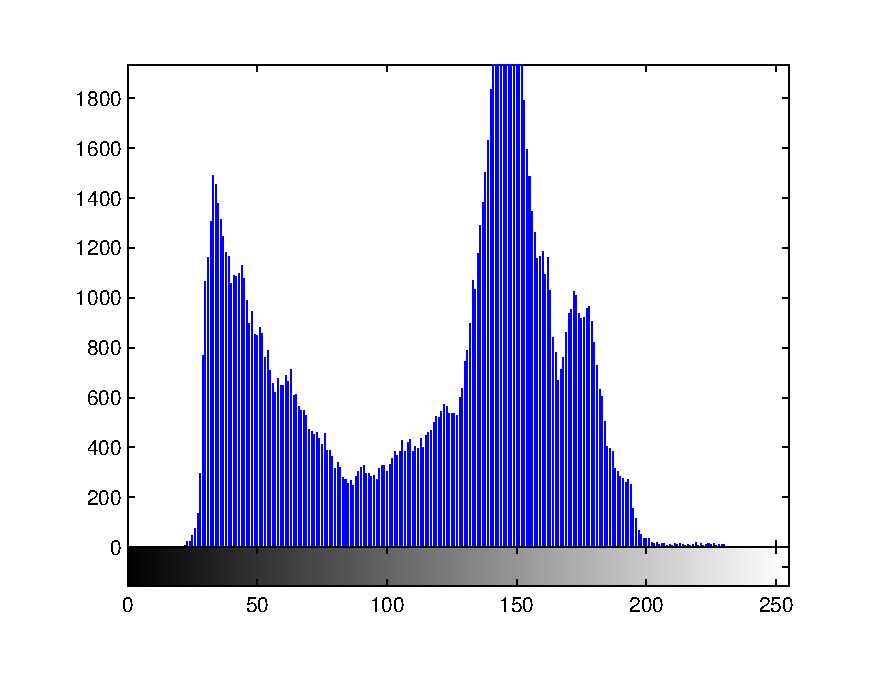
\includegraphics[width=2.5in]{unequalized.eps}
\caption{未均衡的图像的直方图}
\label{fig:a}
\end{minipage}%
\begin{minipage}[h]{0.5\linewidth}
\centering
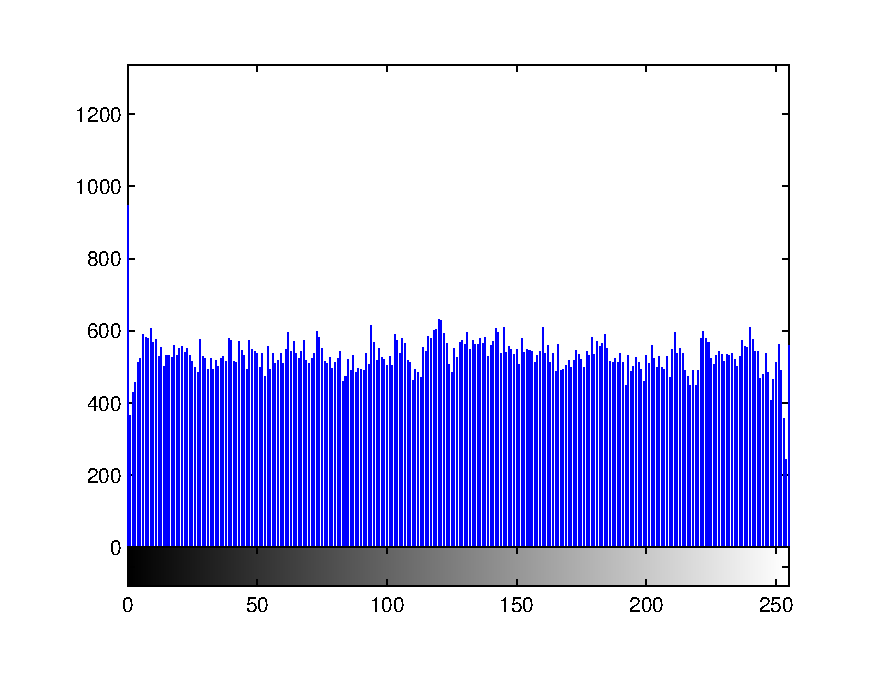
\includegraphics[width=2.5in]{equalized.eps}
\caption{均衡后的图像的直方图}
\label{fig:b}
\end{minipage}
\end{figure}
\bibliographystyle{unsrt}
\bibliography{main}

\end{document}
